\documentclas\documentclass[aspectratio=169,11pt]{beamer}

\usepackage[spanish,es-nodecimaldot]{babel}
\usepackage{amsmath,amssymb,graphicx}
\usepackage{lmodern}
\usepackage{pgfplots}
\pgfplotsset{compat=1.18}

% Paleta en variaciones de azul
\definecolor{AzulNoche}{HTML}{082F49}
\definecolor{AzulProfundo}{HTML}{0C4A6E}
\definecolor{AzulMedio}{HTML}{0369A1}
\definecolor{AzulVivo}{HTML}{0284C7}
\definecolor{AzulClaro}{HTML}{38BDF8}
\definecolor{AzulHielo}{HTML}{E0F2FE}
\definecolor{Fondo}{HTML}{F8FBFF}
\definecolor{Gris}{HTML}{475569}

\setbeamercolor{normal text}{fg=AzulNoche,bg=Fondo}
\setbeamercolor{structure}{fg=AzulMedio}
\setbeamercolor{frametitle}{fg=AzulNoche,bg=Fondo}
\setbeamercolor{block title}{fg=white,bg=AzulProfundo}
\setbeamercolor{block body}{fg=AzulNoche,bg=AzulHielo}
\setbeamercolor{alerted text}{fg=AzulMedio}
\setbeamertemplate{navigation symbols}{}
\setbeamertemplate{items}[circle]
\setbeamertemplate{frametitle}{%
  \vspace{0.22cm}\insertframetitle\par\vspace{0.05cm}%
  {\color{AzulClaro}\rule{1.30cm}{1.5pt}}}
\setbeamertemplate{footline}{%
  \begin{beamercolorbox}[wd=\paperwidth,ht=2.7ex,dp=1.2ex,leftskip=.55cm,rightskip=.55cm]{author in head/foot}%
  \color{Gris}\scriptsize Acemoglu, Kong y Ozdaglar (2026) - NBER WP 34910
  \hfill\textcolor{AzulMedio}{\insertframenumber/8}
  \end{beamercolorbox}}
\setbeamerfont{title}{size=\fontsize{25}{29}\selectfont,series=\bfseries}
\setbeamerfont{frametitle}{size=\Large,series=\bfseries}
\setbeamerfont{block title}{size=\normalsize,series=\bfseries}

\newcommand{\azul}[1]{\textcolor{AzulMedio}{\textbf{#1}}}
\newcommand{\repo}{\href{https://github.com/isisroquet-mi/ai-04-acemoglu}{github.com/isisroquet-mi/ai-04-acemoglu}}

\pgfplotsset{
  grafico/.style={
    axis lines=left,
    axis line style={AzulNoche,semithick},
    tick style={AzulNoche},
    tick label style={font=\scriptsize,color=AzulNoche},
    label style={font=\scriptsize,color=AzulNoche},
    title style={font=\small\bfseries,color=AzulProfundo},
    legend style={font=\scriptsize,draw=none,fill=none},
    grid=major,
    grid style={AzulHielo},
    clip=false
  }
}

\title{IA, cognición humana y colapso del conocimiento}
\subtitle{Repositorio 4 - Modelo, resultado y lectura crítica}
\author{Isis Roque}
\date{NBER Working Paper No. 34910 - febrero de 2026}

\begin{document}

% 1. Portada
\begingroup
\setbeamercolor{background canvas}{bg=AzulNoche}
\begin{frame}[plain]
  \vfill
  \hspace{0.65cm}\begin{minipage}{0.84\paperwidth}
    {\color{AzulClaro}\rule{1.6cm}{2pt}}\\[0.45cm]
    {\usebeamerfont{title}\color{white}\inserttitle\par}
    \vspace{0.34cm}
    {\large\color{AzulHielo}\insertsubtitle\par}
    \vspace{0.85cm}
    {\normalsize\color{white}\insertauthor\par}
    {\small\color{AzulHielo}\insertdate\par}
    \vspace{0.45cm}
    {\small\color{AzulClaro}\repo}
  \end{minipage}
  \vfill
\end{frame}
\endgroup

% 2. Artículo y problema del agente
\begin{frame}{El artículo y el problema del agente}
\begin{block}{Pregunta}
¿La IA agéntica mejora las decisiones presentes a costa del aprendizaje humano que sostiene el conocimiento colectivo?
\end{block}

\begin{columns}[T,onlytextwidth]
\column{0.56\textwidth}
\azul{Elección privada}
{\small
\[
\begin{aligned}
\max_{e_{i,t}\ge 0}\ U_{i,t}
={}&f(0,0)+G(X_t)\Delta_G\\
&+G(X_t)G(Y_{i,t})\Delta_X-\frac{e_{i,t}^{\alpha}}{\alpha},
\qquad \alpha>1.
\end{aligned}
\]}
\[
Y_{i,t}=\sigma^{-2}+\lambda_I e_{i,t}+\tau_A.
\]

\column{0.40\textwidth}
\azul{Dos conocimientos}
\begin{itemize}\small
  \item $X_t$: conocimiento general heredado y compartido.
  \item $Y_{i,t}$: información específica del contexto.
  \item $e_{i,t}$ produce una señal privada y una señal pública ``delgada''.
\end{itemize}
\end{columns}

\vspace{0.05cm}
{\small\color{Gris}\textbf{Externalidad:} el agente internaliza el beneficio privado de aprender, pero no el aporte de su señal al conocimiento de cohortes futuras.}
\end{frame}

% 3. Resultado principal y condiciones
\begin{frame}{Resultado principal y condiciones}
\begin{columns}[T,onlytextwidth]
\column{0.47\textwidth}
\azul{Tensión estática: Observación 1}
\[
\frac{\partial U}{\partial e}
=\Delta_XG(X)\lambda_I g(Y)-e^{\alpha-1}.
\]
\[
\frac{\partial^2U}{\partial e\,\partial X}
=\Delta_X\lambda_I g(X)g(Y)>0,
\]
\[
\frac{\partial^2U}{\partial e\,\partial\tau_A}
=\Delta_XG(X)\lambda_I g'(Y)<0.
\]
{\small Condiciones: $\Delta_X>0$, $\lambda_I>0$, $g>0$, $g'<0$ y costo convexo $\alpha>1$. Así, $e^*$ aumenta con $X$ y disminuye con $\tau_A$.}

\column{0.49\textwidth}
\azul{Dinámica: cuándo aparece el colapso}
\begin{itemize}\small
  \item Si $\alpha-1>\tfrac14$ ($\varepsilon<4$), todo $X_1>0$ converge al único estado estable de conocimiento alto $\bar X_h>0$.
  \item Si $\alpha-1<\tfrac14$ ($\varepsilon>4$) y $\tau_A<\tau_A^c$, existen $0<\bar X_m<\bar X_h$: $X_1<\bar X_m$ converge a $0$ y $X_1>\bar X_m$ converge a $\bar X_h$.
  \item Si $\alpha-1<\tfrac14$ y $\tau_A>\tau_A^c$, $\bar X=0$ es el único estado estacionario y es globalmente estable.
\end{itemize}
\vspace{0.08cm}
{\footnotesize\color{Gris}El paper usa desigualdades estrictas. El caso frontera $\alpha-1=\tfrac14$ y la igualdad $\tau_A=\tau_A^c$ no forman parte de estas proposiciones.}
\end{columns}
\end{frame}

% 4. Lo que hice
\begin{frame}{Lo que hice}
\begin{columns}[T,onlytextwidth]
\column{0.48\textwidth}
\azul{Lectura y verificación}
\begin{itemize}\footnotesize
  \item Trabajé con el NBER Working Paper No. 34910, febrero de 2026, 69 páginas y no revisado por pares.
  \item Lo contrasté con la versión del 5 de mayo de 2026: mismo título, autores, 69 páginas y argumento central. Cambia la portada, la redacción y la parametrización $\alpha-1$ frente a $\varepsilon=1/(\alpha-1)$.
  \item Derivé la Observación 1 y separé el efecto directo e indirecto de $\tau_A$ sobre el bienestar.
\end{itemize}

\column{0.48\textwidth}
\azul{Qué demuestra y qué supone}
\begin{block}{Demostrado dentro del modelo}
\small La IA agéntica reduce el retorno marginal del esfuerzo. Bajo las condiciones de elasticidad y precisión, puede eliminar el equilibrio de conocimiento alto.
\end{block}
\begin{block}{Dependencia crítica de supuestos}
\small La Sección 5 relaja agregación, datos sintéticos y separabilidad imperfecta, pero mantiene $\Delta_I=0$ y $\Delta_X>0$. Con $\Delta_I>0$, la información específica podría conservar valor aun con poco conocimiento general.
\end{block}
\end{columns}
\end{frame}

% 5. Dónde no creí en la IA
\begin{frame}{Dónde no creí en la IA}
\begin{columns}[T,onlytextwidth]
\column{0.42\textwidth}
\azul{La intuición que puse a prueba}

{\footnotesize ``Más precisión de la IA siempre aumenta el bienestar.''}

\vspace{-0.03cm}
{\scriptsize
\[
\begin{aligned}
\frac{d\bar U^+}{d\tau_A}
={}&\underbrace{G(\bar X_h)\Delta_Xg(\bar Y_h)}_{\text{directo }>0}\\
&+\underbrace{g(\bar X_h)\big[\Delta_G+G(\bar Y_h)\Delta_X\big]
\frac{d\bar X_h}{d\tau_A}}_{\text{indirecto }<0}.
\end{aligned}
\]}
{\tiny Con el Supuesto 2, $\sigma^{-2}\ge\sqrt2-1$, $\bar U^+(\tau_A)$ tiene un pico único.}\par
\vspace{0.02cm}
{\scriptsize\color{AzulProfundo}\textbf{Veredicto: incompleta.} El efecto indirecto puede dominar.}

\column{0.54\textwidth}
\centering
\IfFileExists{hand/Derivación_Manual.pdf}{%
  \fcolorbox{AzulClaro}{white}{\includegraphics[page=3,width=0.96\linewidth,height=0.61\textheight,trim=30 425 30 28,clip,keepaspectratio]{hand/Derivación_Manual.pdf}}%
}{%
  \IfFileExists{derivacion-bienestar.png}{%
    \fcolorbox{AzulClaro}{white}{\includegraphics[width=0.96\linewidth,height=0.61\textheight,trim=80 520 80 35,clip,keepaspectratio]{derivacion-bienestar.png}}%
  }{%
    \fcolorbox{AzulClaro}{white}{\parbox[c][0.55\textheight][c]{0.92\linewidth}{\centering\color{Gris}Inserte aquí la página 3 de la derivación manual.}}%
  }%
}

{\tiny\color{Gris}Derivación manual de Isis Roque, p.~3: efecto directo $>0$ e indirecto $<0$.}
\end{columns}
\end{frame}

% 6. Dinámica y alpha
\begin{frame}{Dinámica: el papel de $\alpha$}
\vspace{-0.08cm}
{\footnotesize Los estados estacionarios aparecen donde $F(X)$ corta la línea de 45 grados. Se fija $\tau_A=0.50$ y se modifica únicamente $\alpha$.}

\begin{columns}[T,onlytextwidth]
\column{0.49\textwidth}
\centering
\begin{tikzpicture}
\begin{axis}[
  grafico,width=\linewidth,height=0.50\textheight,
  xmin=0,xmax=0.62,ymin=0,ymax=0.62,
  xtick={0,0.2,0.4,0.6},ytick={0,0.2,0.4,0.6},
  xlabel={$X_t$},ylabel={$X_{t+1}$},
  title={$\alpha=1.50$: equilibrio alto único}
]
\addplot[AzulClaro,densely dashed,semithick] coordinates {(0,0) (0.62,0.62)};
\addplot[AzulProfundo,very thick,smooth] coordinates {
(0.000,0.0000) (0.025,0.0805) (0.050,0.1435) (0.075,0.1947)
(0.100,0.2374) (0.125,0.2738) (0.150,0.3053) (0.175,0.3330)
(0.200,0.3577) (0.225,0.3797) (0.250,0.3997) (0.275,0.4178)
(0.300,0.4344) (0.325,0.4497) (0.350,0.4638) (0.375,0.4770)
(0.400,0.4892) (0.425,0.5007) (0.450,0.5114) (0.475,0.5215)
(0.500,0.5311) (0.525,0.5401) (0.550,0.5486) (0.575,0.5567)
(0.600,0.5645)};
\addplot[only marks,mark=*,mark size=2.2pt,AzulProfundo] coordinates {(0.5479,0.5479)};
\node[font=\scriptsize,anchor=west,text=AzulProfundo] at (axis cs:0.555,0.5479) {$\bar X_h$};
\end{axis}
\end{tikzpicture}

\column{0.49\textwidth}
\centering
\begin{tikzpicture}
\begin{axis}[
  grafico,width=\linewidth,height=0.50\textheight,
  xmin=0,xmax=0.62,ymin=0,ymax=0.62,
  xtick={0,0.2,0.4,0.6},ytick={0,0.2,0.4,0.6},
  xlabel={$X_t$},ylabel={$X_{t+1}$},
  title={$\alpha=1.20$: tres estados estacionarios}
]
\addplot[AzulClaro,densely dashed,semithick] coordinates {(0,0) (0.62,0.62)};
\addplot[AzulVivo,very thick,smooth] coordinates {
(0.000,0.0000) (0.025,0.0248) (0.050,0.0496) (0.075,0.0749)
(0.100,0.1006) (0.125,0.1265) (0.150,0.1524) (0.175,0.1781)
(0.200,0.2033) (0.225,0.2278) (0.250,0.2514) (0.275,0.2741)
(0.300,0.2957) (0.325,0.3162) (0.350,0.3357) (0.375,0.3541)
(0.400,0.3716) (0.425,0.3880) (0.450,0.4036) (0.475,0.4183)
(0.500,0.4323) (0.525,0.4455) (0.550,0.4580) (0.575,0.4699)
(0.600,0.4811)};
\addplot[only marks,mark=*,mark size=2.2pt,AzulProfundo] coordinates {(0,0) (0.2664,0.2664)};
\addplot[only marks,mark=o,mark size=2.4pt,very thick,AzulClaro] coordinates {(0.0804,0.0804)};
\node[font=\scriptsize,anchor=south west,text=AzulMedio] at (axis cs:0.092,0.0804) {$\bar X_m$};
\node[font=\scriptsize,anchor=west,text=AzulProfundo] at (axis cs:0.276,0.2664) {$\bar X_h$};
\end{axis}
\end{tikzpicture}
\end{columns}

\vspace{-0.08cm}
{\footnotesize $\alpha=1.50$ cumple $\alpha-1>\tfrac14$: $0$ es inestable. Con $\alpha=1.20$, $\alpha-1<\tfrac14$ y aparece el umbral inestable $\bar X_m$.}

{\tiny\color{Gris}Simulación ilustrativa: $\Delta_X=6$, $\lambda_I=I=\Sigma^2=1$, $\lambda_G=2$ y $\sigma^{-2}=0.5$.}
\end{frame}

% 7. Umbral de colapso
\begin{frame}{Umbral de colapso}
\begin{columns}[T,onlytextwidth]
\column{0.66\textwidth}
\centering
\begin{tikzpicture}
\begin{axis}[
  grafico,width=\linewidth,height=0.58\textheight,
  xmin=0,xmax=0.62,ymin=0,ymax=0.62,
  xtick={0,0.2,0.4,0.6},ytick={0,0.2,0.4,0.6},
  xlabel={$X_t$},ylabel={$X_{t+1}$},
  legend style={font=\tiny,at={(0.02,0.98)},anchor=north west,row sep=-1pt}
]
\addplot[Gris,densely dashed,semithick] coordinates {(0,0) (0.62,0.62)};
\addlegendentry{Línea de 45 grados}
\addplot[AzulProfundo,very thick,smooth] coordinates {
(0.000,0.0000) (0.025,0.0259) (0.050,0.0552) (0.075,0.0882)
(0.100,0.1238) (0.125,0.1603) (0.150,0.1962) (0.175,0.2304)
(0.200,0.2625) (0.225,0.2923) (0.250,0.3197) (0.275,0.3448)
(0.300,0.3679) (0.325,0.3891) (0.350,0.4087) (0.375,0.4267)
(0.400,0.4434) (0.425,0.4589) (0.450,0.4732) (0.475,0.4867)
(0.500,0.4992) (0.525,0.5109) (0.550,0.5220) (0.575,0.5324)
(0.600,0.5422)};
\addlegendentry{$\tau_A=0.25<\tau_A^c$}
\addplot[AzulVivo,very thick,densely dotted,smooth] coordinates {
(0.000,0.0000) (0.025,0.0247) (0.050,0.0494) (0.075,0.0743)
(0.100,0.0994) (0.125,0.1247) (0.150,0.1500) (0.175,0.1750)
(0.200,0.1995) (0.225,0.2234) (0.250,0.2465) (0.275,0.2687)
(0.300,0.2900) (0.325,0.3102) (0.350,0.3295) (0.375,0.3478)
(0.400,0.3652) (0.425,0.3816) (0.450,0.3972) (0.475,0.4119)
(0.500,0.4259) (0.525,0.4392) (0.550,0.4517) (0.575,0.4637)
(0.600,0.4751)};
\addlegendentry{$\tau_A=\tau_A^c\approx0.526$}
\addplot[AzulClaro,very thick,densely dashed,smooth] coordinates {
(0.000,0.0000) (0.025,0.0247) (0.050,0.0492) (0.075,0.0738)
(0.100,0.0985) (0.125,0.1233) (0.150,0.1480) (0.175,0.1724)
(0.200,0.1964) (0.225,0.2198) (0.250,0.2424) (0.275,0.2643)
(0.300,0.2852) (0.325,0.3052) (0.350,0.3243) (0.375,0.3424)
(0.400,0.3597) (0.425,0.3761) (0.450,0.3916) (0.475,0.4064)
(0.500,0.4204) (0.525,0.4337) (0.550,0.4463) (0.575,0.4583)
(0.600,0.4697)};
\addlegendentry{$\tau_A=0.55>\tau_A^c$}
\addplot[only marks,mark=*,mark size=2.1pt,AzulVivo] coordinates {(0.1633,0.1633)};
\end{axis}
\end{tikzpicture}

\column{0.30\textwidth}
\azul{Desplazamiento de $F(X)$}

{\footnotesize Se mantiene $\alpha=1.20$. Al aumentar $\tau_A$, el esfuerzo humano cae y todo el mapa $F$ se desplaza hacia abajo.}

\vspace{0.15cm}
{\normalsize
\[
\tau_A^c\approx0.526.
\]}

\begin{itemize}\scriptsize
  \item Por debajo, existen dos equilibrios positivos.
  \item En el umbral, ambos se unen por tangencia.
  \item Por encima, solo queda el colapso $\bar X=0$.
\end{itemize}
\end{columns}
\end{frame}

% 8. Path dependence
\begin{frame}{Dependencia de la condición inicial}
\begin{columns}[T,onlytextwidth]
\column{0.70\textwidth}
\centering
\begin{tikzpicture}
\begin{axis}[
  grafico,width=\linewidth,height=0.60\textheight,
  xmin=0,xmax=400,ymin=0,ymax=0.30,
  xtick={0,100,200,300,400},ytick={0,0.1,0.2,0.3},
  xlabel={Cohorte, $t$},ylabel={Conocimiento general, $X_t$},
  legend style={at={(0.97,0.52)},anchor=east,row sep=1pt}
]
\addplot[AzulClaro,densely dashed,semithick] coordinates {(0,0.0804) (400,0.0804)};
\addlegendentry{Umbral $\bar X_m=0.0804$}
\addplot[AzulProfundo,very thick,smooth] coordinates {
(0,0.07000) (20,0.06543) (40,0.05960) (60,0.05275) (80,0.04542)
(100,0.03828) (120,0.03188) (140,0.02649) (160,0.02212)
(180,0.01864) (200,0.01589) (220,0.01370) (240,0.01195)
(260,0.01053) (280,0.00937) (300,0.00841) (320,0.00760)
(340,0.00692) (360,0.00634) (380,0.00584) (400,0.00540)};
\addlegendentry{$X_1=0.07<\bar X_m$}
\addplot[AzulVivo,very thick,smooth] coordinates {
(0,0.09000) (20,0.09649) (40,0.10860) (60,0.13330) (80,0.18371)
(100,0.24244) (120,0.26286) (140,0.26597) (160,0.26635)
(180,0.26640) (200,0.26641) (220,0.26641) (240,0.26641)
(260,0.26641) (280,0.26641) (300,0.26641) (320,0.26641)
(340,0.26641) (360,0.26641) (380,0.26641) (400,0.26641)};
\addlegendentry{$X_1=0.09>\bar X_m$}
\addplot[AzulMedio,densely dotted,semithick] coordinates {(0,0.2664) (400,0.2664)};
\end{axis}
\end{tikzpicture}

\column{0.26\textwidth}
{\footnotesize Con $\alpha=1.20$ y $\tau_A=0.50$ existen tres estados estacionarios:}
{\small
\[
\begin{aligned}
\bar X_m&\approx0.0804,\\
\bar X_h&\approx0.2664.
\end{aligned}
\]}
\begin{itemize}\scriptsize
  \item $X_1=0.07$ cae gradualmente hacia $0$.
  \item $X_1=0.09$ converge hacia $\bar X_h$.
\end{itemize}

{\tiny\color{Gris}El umbral separa dos cuencas de atracción. Una diferencia inicial de $0.02$ cambia el resultado de largo plazo.}
\end{columns}
\end{frame}

\end{document}

\definecolor{PaleGold}{HTML}{F5EBD5}
\definecolor{CodeBg}{HTML}{F1F3F5}

\setbeamercolor{normal text}{fg=Ink,bg=Paper}
\setbeamercolor{structure}{fg=Teal}
\setbeamercolor{frametitle}{fg=white,bg=Navy}
\setbeamercolor{title}{fg=white}
\setbeamercolor{subtitle}{fg=PaleTeal}
\setbeamercolor{alerted text}{fg=Teal}
\setbeamercolor{itemize item}{fg=Gold}
\setbeamercolor{enumerate item}{fg=Gold}
\setbeamercolor{block title}{fg=white,bg=Teal}
\setbeamercolor{block body}{fg=Ink,bg=PaleTeal}

\setbeamerfont{title}{series=\bfseries,size=\LARGE}
\setbeamerfont{subtitle}{size=\large}
\setbeamerfont{frametitle}{series=\bfseries,size=\Large}
\setbeamerfont{footline}{size=\scriptsize}
\setbeamertemplate{navigation symbols}{}
\setbeamertemplate{itemize item}{\raise0.15ex\hbox{\color{Gold}$\blacktriangleright$}}
\setbeamertemplate{itemize subitem}{\raise0.1ex\hbox{\color{Teal}$\bullet$}}
\setbeamertemplate{frametitle}{%
  \nointerlineskip
  \begin{beamercolorbox}[wd=\paperwidth,ht=0.84cm,dp=0.22cm,leftskip=0.65cm,rightskip=0.35cm]{frametitle}
    \usebeamerfont{frametitle}\insertframetitle
  \end{beamercolorbox}}
\setbeamertemplate{footline}{%
  \leavevmode\hbox{%
    \begin{beamercolorbox}[wd=.86\paperwidth,ht=0.32cm,dp=0.12cm,leftskip=.55cm]{author in head/foot}%
      \color{Muted}Quispe y Xu (2026) \;\textbar\; IA y Modelamiento Económico
    \end{beamercolorbox}%
    \begin{beamercolorbox}[wd=.14\paperwidth,ht=0.32cm,dp=0.12cm,rightskip=.45cm plus1fil]{date in head/foot}%
      \color{Muted}\hfill\insertframenumber/\inserttotalframenumber
    \end{beamercolorbox}}}
\setbeamertemplate{headline}{}

\hypersetup{colorlinks=true,urlcolor=Teal,linkcolor=Teal}
\newcommand{\key}[1]{\textcolor{Teal}{\textbf{#1}}}
\newcommand{\source}[1]{\par\vfill{\fontsize{6.2}{7.2}\selectfont\color{Muted}Fuente: #1}}
\lstdefinelanguage{Lean}{
  morekeywords={def,theorem,by,intro,unfold,rw,simp,only,Prop,Real},
  sensitive=true,morecomment=[l]{--},morestring=[b]"
}
\lstset{language=Lean,basicstyle=\ttfamily\fontsize{7.2}{8.4}\selectfont,
  keywordstyle=\bfseries\color{Teal},commentstyle=\itshape\color{Muted},
  backgroundcolor=\color{CodeBg},frame=single,rulecolor=\color{PaleTeal},
  showstringspaces=false,columns=fullflexible,keepspaces=true,breaklines=true,
  xleftmargin=0.15em,xrightmargin=0.15em,aboveskip=0.25em,belowskip=0.25em}

\title{Claude Code y la frontera tecnológica del desarrollador}
\subtitle{Quispe y Xu (2026): resultado, verificación y límite causal}
\author{Alexander Quispe}
\institute{IA y Modelamiento Económico \;\textbar\; Universidad del Pacífico}
\date{Tarea 2 \;\textbar\; 2026}

\begin{document}

{\setbeamercolor{background canvas}{bg=Navy}
\begin{frame}[plain]
    \vspace*{1.1cm}\hspace*{0.75cm}\begin{minipage}{0.84\paperwidth}
      {\color{Gold}\rule{1.45cm}{2.2pt}}\\[0.55cm]
      {\usebeamerfont{title}\color{white}\inserttitle\par}
      \vspace{0.25cm}{\usebeamerfont{subtitle}\color{PaleTeal}\insertsubtitle\par}
      \vspace{0.85cm}{\color{white}\large\insertauthor\par}
      \vspace{0.12cm}{\color{PaleTeal}\insertinstitute\par}
      \vspace{0.12cm}{\color{PaleTeal}\insertdate\par}
      \vspace{0.75cm}{\small\color{white}\href{https://github.com/isisroquet-mi/ai-03-quispe}{github.com/isisroquet-mi/ai-03-quispe}}
    \end{minipage}
\end{frame}
}

\begin{frame}{Pregunta: ¿productividad o expansión de frontera?}
  \begin{columns}[T,onlytextwidth]
    \begin{column}{0.56\textwidth}
      \vspace{0.15cm}
      \textbf{Objeto económico.} La frontera de producción es el conjunto de lenguajes en los que el desarrollador logra producir código, aunque no los dominara previamente.
      \vspace{0.42cm}
      \begin{block}{Pregunta del documento}
        ¿La adopción de Claude Code permite activar lenguajes que antes quedaban fuera del portafolio observado?
      \end{block}
      \vspace{0.25cm}
      La predicción se evalúa en cuatro márgenes: lenguajes activos, lenguajes nuevos, diversidad y acumulación del portafolio.
    \end{column}
    \begin{column}{0.39\textwidth}
      \centering\vspace{0.15cm}
      {\color{Muted}\small habilidad previa}\\[0.18cm]
      {\Large $\mathcal{L}^{\text{habilidad}}_i$}\\[0.35cm]
      {\color{Gold}\LARGE $\Downarrow$}\\[0.28cm]
      \colorbox{PaleTeal}{\parbox[c][1.65cm][c]{0.88\linewidth}{\centering
        {\color{Teal}\bfseries delegación agentic}\\[-0.05cm]reduce el umbral de entrada}}
      \\[0.28cm]{\color{Gold}\LARGE $\Downarrow$}\\[0.18cm]
      {\Large $\mathcal{L}^{\text{producción}}_i$}\\[0.18cm]
      {\color{Muted}\small portafolio observado}
    \end{column}
  \end{columns}
  \source{Quispe y Xu (2026), \emph{Coding Beyond Your Training: Claude Code and the Technological Frontier of Software Developers}.}
\end{frame}

\begin{frame}{La comparación exigida: una decisión de modelamiento}
  \begin{columns}[T,onlytextwidth]
    \begin{column}{0.47\textwidth}
      {\color{Teal}\Large\bfseries Quispe--Xu}\\[0.18cm]
      \textbf{IA como señal y capacidad de ejecución.}
      \begin{itemize}
        \item Añade el modo de delegación $D$ al menú del agente.
        \item Puede bajar el umbral para lenguajes desconocidos.
        \item Predice \key{expansión de la frontera de producción}.
      \end{itemize}
      \[M^1=\{S,C\}\ \longrightarrow\ M^2=\{S,C,D\}\]
    \end{column}
    \begin{column}{0.045\textwidth}
      \centering\vspace{0.35cm}{\color{Gold}\rule{1pt}{4.45cm}}
    \end{column}
    \begin{column}{0.47\textwidth}
      {\color{Navy}\Large\bfseries Aouad--Lykouris--Zhong}\\[0.18cm]
      \textbf{IA como insumo perfectamente sustituible.}
      \begin{itemize}
        \item Habilidad, esfuerzo e IA entran por su suma.
        \item La asistencia desplaza esfuerzo o aprendizaje humano.
        \item Predice \textbf{pérdida o depreciación de habilidades}.
      \end{itemize}
      \[x=s+e+a\]
    \end{column}
  \end{columns}
  \vspace{0.18cm}\centering
  \colorbox{PaleGold}{\parbox{0.92\linewidth}{\centering\bfseries
    Mismo fenómeno tecnológico, conclusiones opuestas: el mecanismo supuesto determina la predicción.}}
  \source{Comparación indicada en las instrucciones de la Tarea 2.}
\end{frame}

\begin{frame}{Problema del agente: elegir modo y activar un lenguaje}
  \begin{columns}[T,onlytextwidth]
    \begin{column}{0.54\textwidth}
      \textbf{Menú antes y después de Claude Code}
      \[M^1=\{S,C\},\qquad M^2=\{S,C,D\}.\]
      Para desarrollador $i$, lenguaje $k$ y período $t$:
      \[V^g_{ik,t}=\max_{m\in M^g}V^m_{ik,t},\qquad
        Z^g_{ik,t}=\mathbf 1\!\left[V^g_{ik,t}\ge0\right].\]
      El número de lenguajes producidos es
      \[N^g_{it}=\sum_k Z^g_{ik,t}.\]
    \end{column}
    \begin{column}{0.41\textwidth}
      \begin{block}{Tres modos}
        \begin{tabular}{@{}>{\bfseries}c p{0.75\linewidth}@{}}
          $S$ & producción sin asistencia;\\[0.16cm]
          $C$ & asistencia conversacional, complementaria a habilidad previa;\\[0.16cm]
          $D$ & delegación agentic de una fracción $\lambda$ de la ejecución.
        \end{tabular}
      \end{block}
      \vspace{0.25cm}
      \textbf{Mecanismo mínimo:} ampliar el menú nunca reduce el valor máximo; la cuestión sustantiva es cuándo $D$ vuelve viable una oportunidad antes inactiva.
    \end{column}
  \end{columns}
\end{frame}

\begin{frame}{De excedentes a umbrales de entrada}
  \begin{columns}[T,onlytextwidth]
    \begin{column}{0.47\textwidth}
      \textbf{Solo y asistencia conversacional}
      \begin{align*}
        V^S&=\omega+s\mu-\frac{\rho s^2}{2\pi}-b,&
        T^S&=b-s\mu+\frac{\rho s^2}{2\pi},\\
        V^C&=V^S+\gamma s-r_C,&
        T^C&=T^S-(\gamma s-r_C),\\
        T^1&=\min\{T^S,T^C\}.&&
      \end{align*}
      Para un lenguaje desconocido:
      \[\gamma s-r_C\le0\quad\Longrightarrow\quad \boxed{T^1=T^S}.\]
    \end{column}
    \begin{column}{0.49\textwidth}
      \textbf{Delegación agentic}
      \[
      \begin{aligned}
        T^D={}&b-(1-\lambda)s\mu-\lambda az(A)+\kappa(a,s)+r_D\\
              &+\frac{\rho}{2}\left[(1-\lambda)^2\frac{s^2}{\pi}
              +\sigma_D^2(a,s,A)\right].
      \end{aligned}
      \]
      Después de Claude Code:
      \[\boxed{T^2=\min\{T^1,T^D\}\le T^1}.\]
      \small
      La desigualdad es débil porque el agente puede ignorar $D$. Para obtener una expansión estricta se necesita algo más que ampliar el menú.
    \end{column}
  \end{columns}
\end{frame}

\begin{frame}{Resultado principal: ganancia de umbral y condiciones}
  \vspace{-0.06cm}
  Para lenguajes desconocidos, defina $B\equiv T^S-T^D$:
  \[
  \boxed{B=\lambda[az(A)-s\mu]-\kappa(a,s)-r_D
  +\frac{\rho}{2}\left[(2\lambda-\lambda^2)\frac{s^2}{\pi}-\sigma_D^2(a,s,A)\right]}
  \]
  \begin{columns}[T,onlytextwidth]
    \begin{column}{0.49\textwidth}
      \textbf{Condiciones económicas y de dominio}
      \begin{enumerate}
        \item $\pi>0$, $\rho\ge0$, $0\le\lambda\le1$ y $\sigma_D^2\ge0$.
        \item $\gamma s-r_C\le0$, de modo que $T^1=T^S$ en lenguajes desconocidos.
        \item $B>0$, equivalente a $T^D<T^S$: el beneficio neto de delegar domina verificación, uso y riesgo residual.
      \end{enumerate}
    \end{column}
    \begin{column}{0.47\textwidth}
      \textbf{Condiciones para observar el efecto}
      \begin{enumerate}\setcounter{enumi}{3}
        \item La oportunidad satisface $T^D\le\omega<T^S$.
        \item Cada $F_k$ es una CDF monótona.
        \item Para una expansión \emph{estricta}, existe masa positiva en al menos una banda: $F_k(T^S_k)>F_k(T^D_k)$.
      \end{enumerate}
    \end{column}
  \end{columns}
\end{frame}

\begin{frame}{Banda de activación y expansión esperada}
  \begin{columns}[T,onlytextwidth]
    \begin{column}{0.42\textwidth}
      \textbf{Tres regiones de oportunidad}\vspace{0.3cm}
      \begin{tabular}{@{}>{\raggedleft\arraybackslash}p{0.35\linewidth}p{0.58\linewidth}@{}}
        $\omega<T^D$ & inactivo incluso con delegación;\\[0.34cm]
        \colorbox{PaleGold}{$T^D\le\omega<T^S$} & \textbf{activo solo con el agente};\\[0.34cm]
        $\omega\ge T^S$ & ya era viable antes.
      \end{tabular}
      \vspace{0.45cm}
      \[Z^2_k-Z^1_k=\mathbf 1[T^D_k\le\omega_k<T^S_k].\]
    \end{column}
    \begin{column}{0.54\textwidth}
      \textbf{De un lenguaje al portafolio}
      \begin{align*}
        \mathbb E[Z^g_k]&=\Pr(\omega_k\ge T^g_k)=1-F_k(T^g_k),\\[0.15cm]
        \mathbb E[N^2-N^1]&=\sum_k\left[F_k(T^1_k)-F_k(T^2_k)\right]\ge0.
      \end{align*}
      Para lenguajes desconocidos con $T^1=T^S$ y $T^2=T^D$:
      \[\boxed{\mathbb E[N^2-N^1]
        =\sum_{k\in U_i}\left[F_k(T^S_k)-F_k(T^D_k)\right]\ge0.}\]
      \small
      El signo débil proviene de la expansión del menú; el signo estricto exige masa de oportunidades dentro de la banda.
    \end{column}
  \end{columns}
\end{frame}

\begin{frame}{Qué hice analítica y computacionalmente}
  \begin{columns}[T,onlytextwidth]
    \begin{column}{0.48\textwidth}
      {\color{Teal}\Large\bfseries Analítico}
      \begin{itemize}
        \item Derivé $T^S$, $T^C$ y $T^D$ desde cada condición $V^m\ge0$.
        \item Expandí manualmente $B=T^S-T^D$ y verifiqué el término de riesgo $2\lambda-\lambda^2$.
        \item Separé expansión débil del menú de expansión estricta con masa positiva.
        \item Identifiqué la banda exacta $T^D\le\omega<T^S$.
      \end{itemize}
    \end{column}
    \begin{column}{0.48\textwidth}
      {\color{Navy}\Large\bfseries Computacional}
      \begin{itemize}
        \item Traduje umbrales, activación y CDF monótona a Lean 4.
        \item Verifiqué identidad algebraica, monotonía del mínimo, equivalencia $B>0\leftrightarrow T^D<T^S$ y banda de activación.
        \item Elaboré la superficie probada con \textbf{0 errores, 0 mensajes} y sin \texttt{sorry}, \texttt{admit} ni axiomas propios.
        \item Conservé el alcance honesto: formalización parcial del mecanismo, no de la identificación empírica.
      \end{itemize}
    \end{column}
  \end{columns}
  \vspace{0.12cm}\centering\small
  \colorbox{PaleTeal}{\parbox{0.91\linewidth}{\centering
    Artefactos auditables: \texttt{hand/derivacion\_manual.pdf} y \texttt{lean/QX26AgenticDelegation/}.}}
\end{frame}

\begin{frame}[fragile]{Lean: de la afirmación matemática a una prueba verificable}
  \textbf{1. Afirmación matemática original}
  \vspace{-0.06cm}
  \[T^D<T^S\quad\Longrightarrow\quad
    \bigl((Z^2-Z^1=1)\Longleftrightarrow T^D\le\omega<T^S\bigr).\]
  \vspace{-0.18cm}
  \begin{columns}[T,onlytextwidth]
    \begin{column}{0.57\textwidth}
      \textbf{2. Declaración Lean y fragmento decisivo}
\begin{lstlisting}
def activationBandSpec (opportunity preThreshold
    agentThreshold : Real) : Prop :=
  agentThreshold < preThreshold ->
    (Active opportunity
        (postThreshold preThreshold agentThreshold) /\
      ~ Active opportunity preThreshold <->
      agentThreshold <= opportunity /\
        opportunity < preThreshold)

theorem activation_band ... := by
  intro hLower
  unfold Active postThreshold
  rw [min_eq_right (le_of_lt hLower)]
  simp only [not_le]
\end{lstlisting}
    \end{column}
    \begin{column}{0.40\textwidth}
      \textbf{3. Qué representa y qué verifica}
      \begin{itemize}\small
        \item \texttt{postThreshold} es $\min\{T^S,T^D\}$; con $T^D<T^S$, Lean lo reescribe como $T^D$.
        \item \texttt{Active omega T} significa $T\le\omega$.
        \item No estar activo antes, $\neg(T^S\le\omega)$, se transforma exactamente en $\omega<T^S$.
        \item Lean certifica la \textbf{implicación condicional}; no prueba que Claude Code cause $T^D<T^S$ en los datos.
      \end{itemize}
    \end{column}
  \end{columns}
\end{frame}

\begin{frame}{Donde no creí en la IA: derivación manual y veredicto}
  \begin{columns}[T,onlytextwidth]
    \begin{column}{0.49\textwidth}
      \centering
      \fcolorbox{Navy}{white}{%
        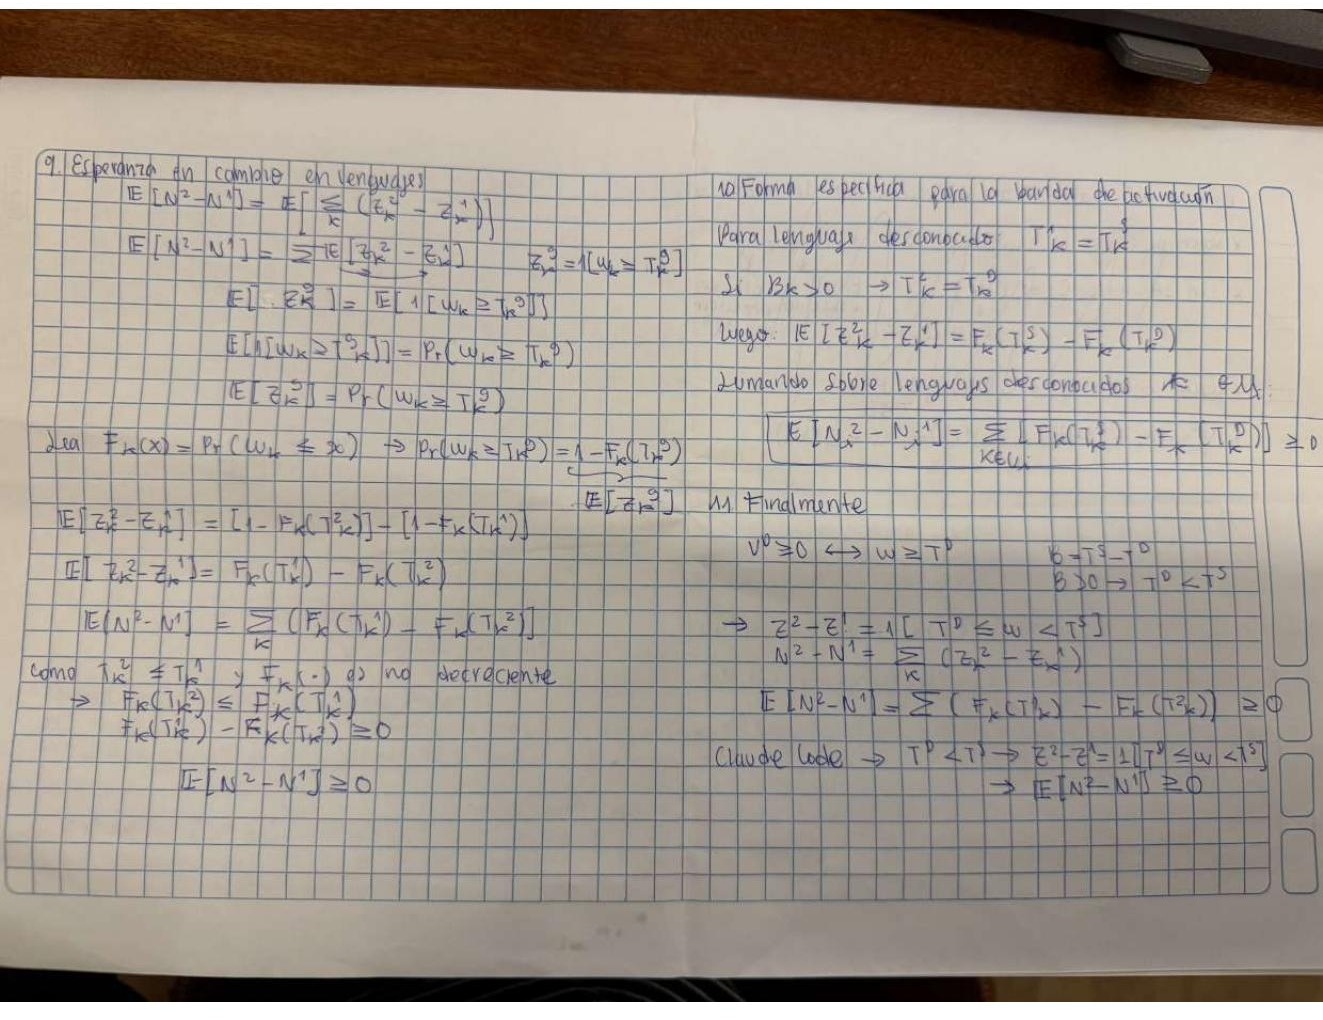
\includegraphics[width=0.95\linewidth]{derivacion_manual_p3_crop.jpg}}
      \\[0.08cm]
      {\scriptsize\color{Muted}Derivación manual: esperanza, banda de activación y signo.}
    \end{column}
    \begin{column}{0.47\textwidth}
      \small
      \textbf{Lo que audité}
      \begin{itemize}
        \item La cancelación algebraica en $B=T^S-T^D$.
        \item La equivalencia exacta entre cambio de activación y banda de oportunidades.
        \item El salto interpretativo entre una predicción condicional y una afirmación causal.
      \end{itemize}
      \vspace{0.06cm}
      \colorbox{PaleGold}{\parbox{0.92\linewidth}{
        \textbf{Veredicto.} La derivación es correcta bajo sus supuestos. La adopción voluntaria es compatible con expansión de frontera, pero no descarta selección: un nuevo proyecto puede inducir tanto la adopción como el nuevo lenguaje.}}
      \vspace{0.18cm}
      \centering\textbf{Mecanismo coherente $\neq$ causalidad identificada.}
    \end{column}
  \end{columns}
\end{frame}

\end{document}
